
\documentclass{article}
\usepackage{graphicx}
\title{COP290 Lab 1- Screen Saver}
\date{25/1/2015}
\author{Akash Tanwar and Aayush Gautam}
\begin{document}
	\maketitle
	\pagenumbering{gobble}
	\newpage
	\pagenumbering{arabic}
	\section{Overall Design}
	This is an \emph{overview} of the final screensaver that we have made.
	\subsection{The User Interface}
	The user interface is developed using openGL\@. It has the look of 3D box with balls moving inside. Every ball has some main properties which are:- radius and mass, velocity and coordinates of its centre. Balls have been formed by running a loop assigning them vertices and forming a polygon with infinite sides which appears like a circle to a normal eye.
	
	The number of balls is given by the user in a specific predefined limit.The velocity of all the balls are random at initialisation. Sizes and velocities can be changed by the user. Their ranges are pre defined. This can be done by right clicking on the screen saver, then selecting the respective ball number and changing its properties. 
		
	Colour of a ball can also be changed by the user. User can also reshape the window.

{\small*Sizes are initialised as equal, unlike velocities.}

	\subsection{Extra Features}
	Variable sizes which means variable mass.	
	
	3D box and viewing facilities.
	
	Variable colour of the balls.

	Screen saver can also be paused. Once the screen saver is paused, everything will stop. The user 	can then move and view the scene and again resume the screensaver whenever he wishes to.

	\section{Sub-Components}
	There are mainly three components being the GUI, physics and managing threads.
	\subsection{GUI}
	Coding with open GL and forming the basic layout of the screensaver with good variable constructs that enable us to make all the features that we have specified. This includes adding textures, making menus, etc.
	\subsection{Physics}
	Making all the formulae of collisions such that the computer can use the `handles' or variables provided by the GUI to solve a collision problem at every instant and calculate how the ball should move.
	
	In our case we have perfectly elastic collisions in 3 dimensions of only two balls. We have assumed that only two balls collide at one instant. Collision of 3 or more balls is assumed to be same as first two balls collide then one by one the other pairs collide. Thus momentum conservation in $x, $y$, $z directions with energy conservation gives us the final velocities of the colliding balls.
	
	In figure 1, the blue ball has velocity $u_1 = u_x^1i+u_y^1j+u_z^1k$ and the red ball has $u_2 = u_x^2i+u_y^2j+u_z^2k$.
	The final velocities after collision are \\[8pt]
	
	$v_1^x=\frac{2*m_2*u_2^x+(m_1-m_2)*u_1^x}{m_1+m_2}$\\[8pt]
	
	
    $v_2^x=\frac{(m_2-m_1)*u_2^x+2*m_1*u_1^x}{m_1+m_2}$\\[8pt]
    
    
    $v_1^y=\frac{2*m_2*u_2^y+(m_1-m_2)*u_1^y}{m_1+m_2}$\\[8pt]
    
    
    $v_2^y=\frac{(m_2-m_1)*u_2^y+2*m_1*u_1^y}{m_1+m_2}$\\[8pt]
    
    
   $v_1^z=\frac{2*m_2*u_2^z+(m_1-m_2)*u_1^z}{m_1+m_2}$\\[8pt]
    
    
    $v_2^z=\frac{(m_2-m_1)*u_2^z+2*m_1*u_1^z}{m_1+m_2}$
    
	\begin{figure}
  	\centering
 	 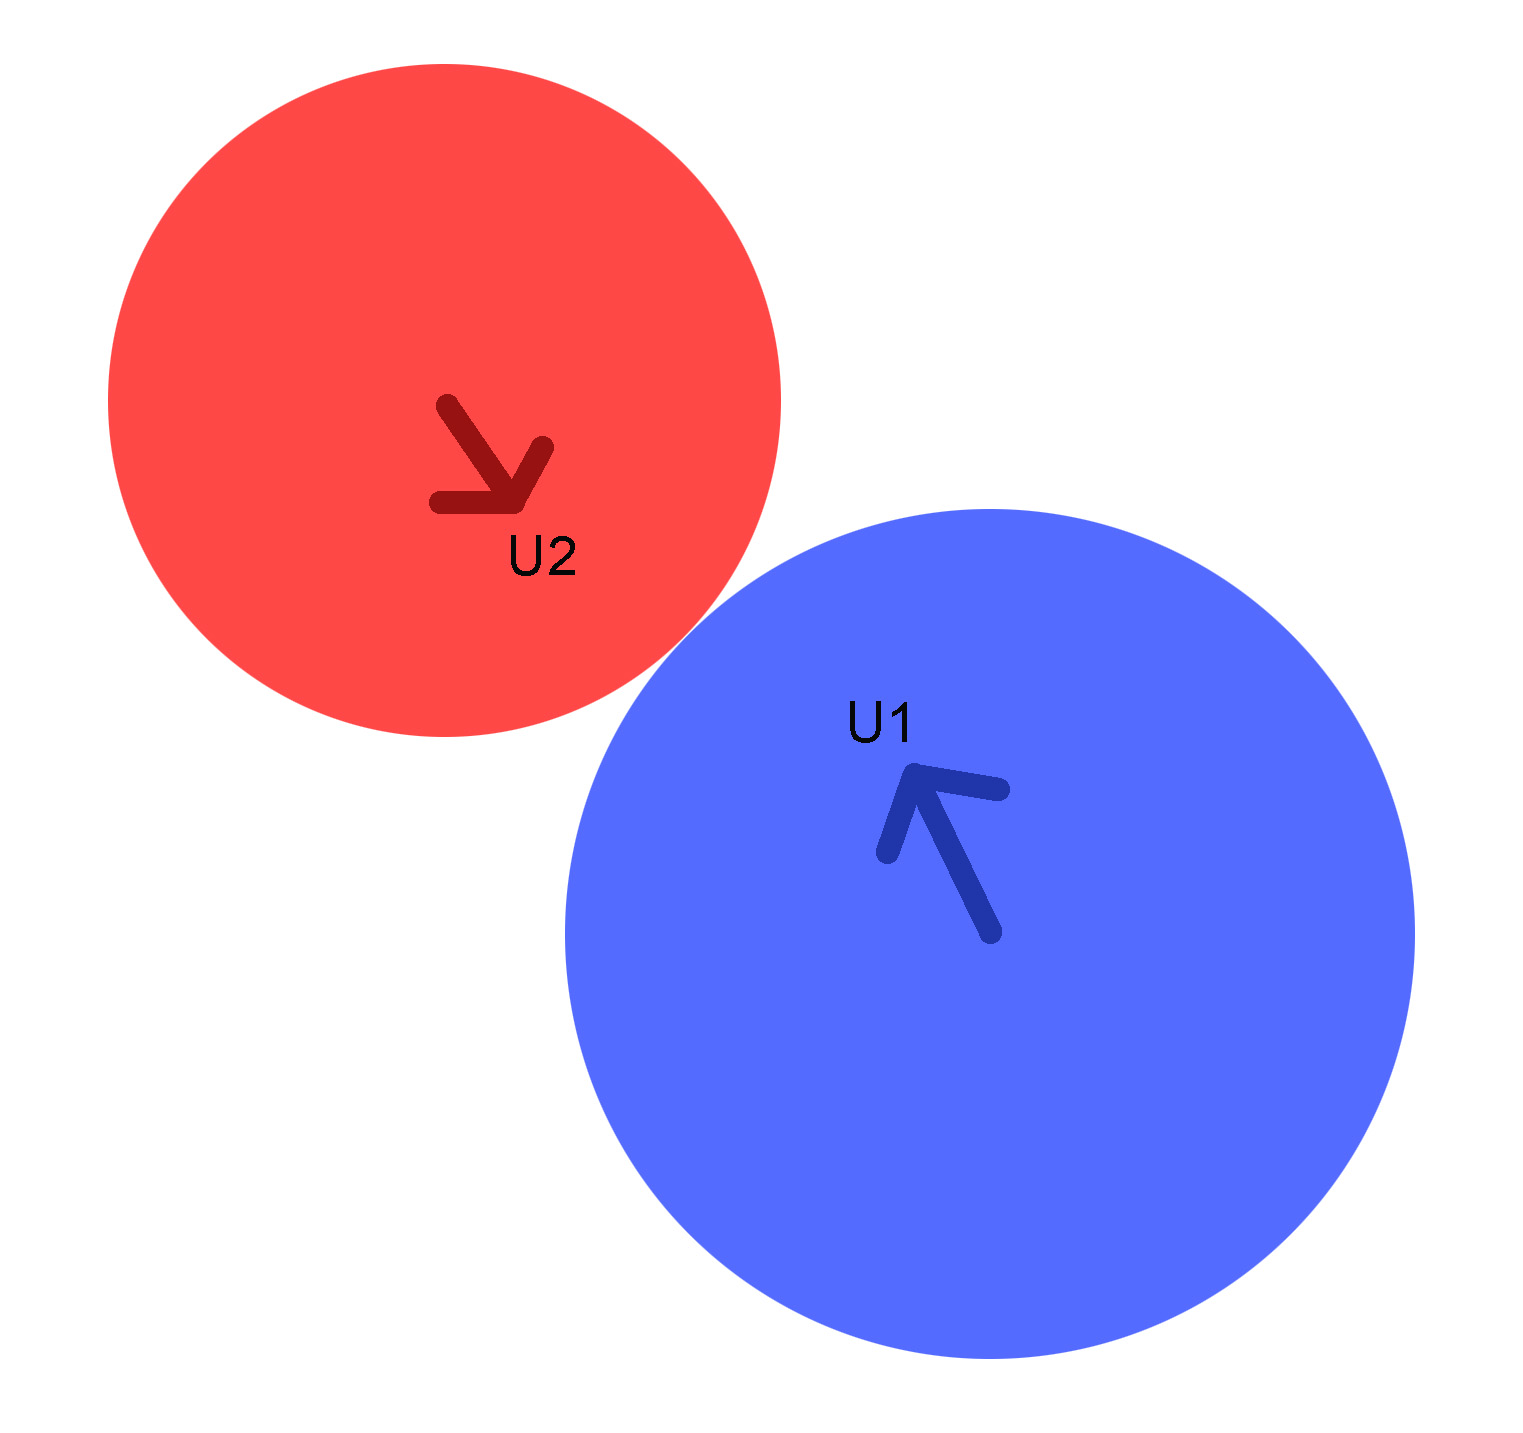
\includegraphics[width=150pt,height=150pt]{diagram.jpg}
	  \caption{3D collision of two balls}
	  \label{fig1}
  	\end{figure}
	
	\subsection{Threads and their synchronisation}
	Using threads (pthreads) to do computations in parallel. The threads will govern the physics functions and manipulate how a ball should move at every instant.
	
	
	\section{Testing of the components}
	We have thought of a three step procedure to test our screen saver.
	\paragraph{1.}
		Running the program and trying all the features many times.
	\paragraph{2.}
		Running Component specific tests that are:-
		\subparagraph{GUI testing}
		GUI can be simply tested by running the program and just observing the interface at first. If everything appears and runs as required then the next step is to start using its features like clicking on the pause button and clicking at random places. After that comes the checking of different front end control handles provided, by using their functions in all the possible cases and observing the changes. If the program doesn't crash and gives the expected results then the GUI is working fine.

		\subparagraph{Threads and physics testing}
		We will have to initialise the balls in specific manners and not randomly as it was before. We will manually code the velocity values such that the balls collide in different manners once the application is launched. In this way all our corner cases of physics and general cases can be observed and tested. If the physics is working right that means our threads are working right because essentially thread's work is to control the physics.
	\paragraph{3.}
	Last thing is to run the program and use all the features that we have discussed above. Try all of them for different number of balls and trying them in their corner cases. After thorough running and trying everything on different systems as well we will be pretty sure that it does not have any loop holes.

	\section{How do the subcomponents interact with each other?}
	GUI interacts with both of the other components and threads interact with the physics component.
	\subsection{Threads and physics}
	Physics is actually just functions to compute final velocities between a colliding pair or a ball colliding with the wall or just move the ball as it was moving. That function is controlled by threads at the right time and in the right way to carry out the respective movements of the bubbles. 
	\subsection{GUI with others}
	GUI produces back end `handles' for programming to run like the ball properties such as velocity components, radius etc.
These handles are controlled by the backend code and produced on the screen.
	\section{How will the threads interact with each other?}
	For a thread to carry out the physics properly, it needs to know the position of the other bubbles too. This is where communication becomes necessary.
	\subsection{Model of interaction}
	We have used one to one synchronisation between the threads.
	\subsection{Mechanism of synchronisation}
	
	\paragraph{}
	Communication will not be fastest or efficient in one to one synchronisation. Every ball's position will be governed by a thread and every ball has its own message queue that will collect the positions and velocities of all the other balls and process it accordingly. 
	\newline
	Simultaneously all the threads will run. Every thread will push its position in the message queues of all the other threads with proper synchronisation using mutex. Then all the threads will start processing the queue and find, if existing, a colliding match. If a colliding match is found then there will be respective change in the velocities of the balls.
	\paragraph{For example}
	Consider 4 bubbles A,B,C and D. A and C are colliding in the scene. 4 threads will start simultaneously searching for their colliding match. Suppose C finds A first. Then C will give its velocity to A. Then it will change its velocity. Then A will find C and make the respective change in itself using the earlier message that it received. B and D will move with the same velocity.
	\paragraph{}
	This is a basic overview of our one to one synchronisation of threads.
	\section{Variable ball speeds}
	 Every ball has its own x, y and z components of velocity, the magnitude of which can be manipulated by the user through our user interface that is a menu to control.

	\section{Changes from the earlier document}
	We made it 3D and changed the design. 
	We also changed the synchronisation model.
\end{document}